\documentclass{article}
\usepackage{fullpage}
\usepackage[normalem]{ulem}
\usepackage{amstext}
\usepackage{amsmath}
\usepackage{bm}
\usepackage{algorithm}
\usepackage[noend]{algpseudocode}
\usepackage{graphicx}
\graphicspath{ {/Users/DanielKong/Desktop/UT/CSC321/Assignments/HW2/HW2 Ans} }
% graph path

%\usepackage{unicode-math}
%\setmathfont{latinmodern-math.otf}
\newcommand{\var}[1]{\mathit{#1}}
\setlength{\parskip}{6pt}

\begin{document}

\noindent
University of Toronto\\
{\sc CSC}321, Winter 2018\\[10pt]
{\LARGE\bf HW 2: Xiangyu Kong 1002109620 kongxi16} \\[10pt]

%----------------------------------------------------------------------------------------------------------------------
\section*{1}

	\begin{figure}[h]
		\centering
		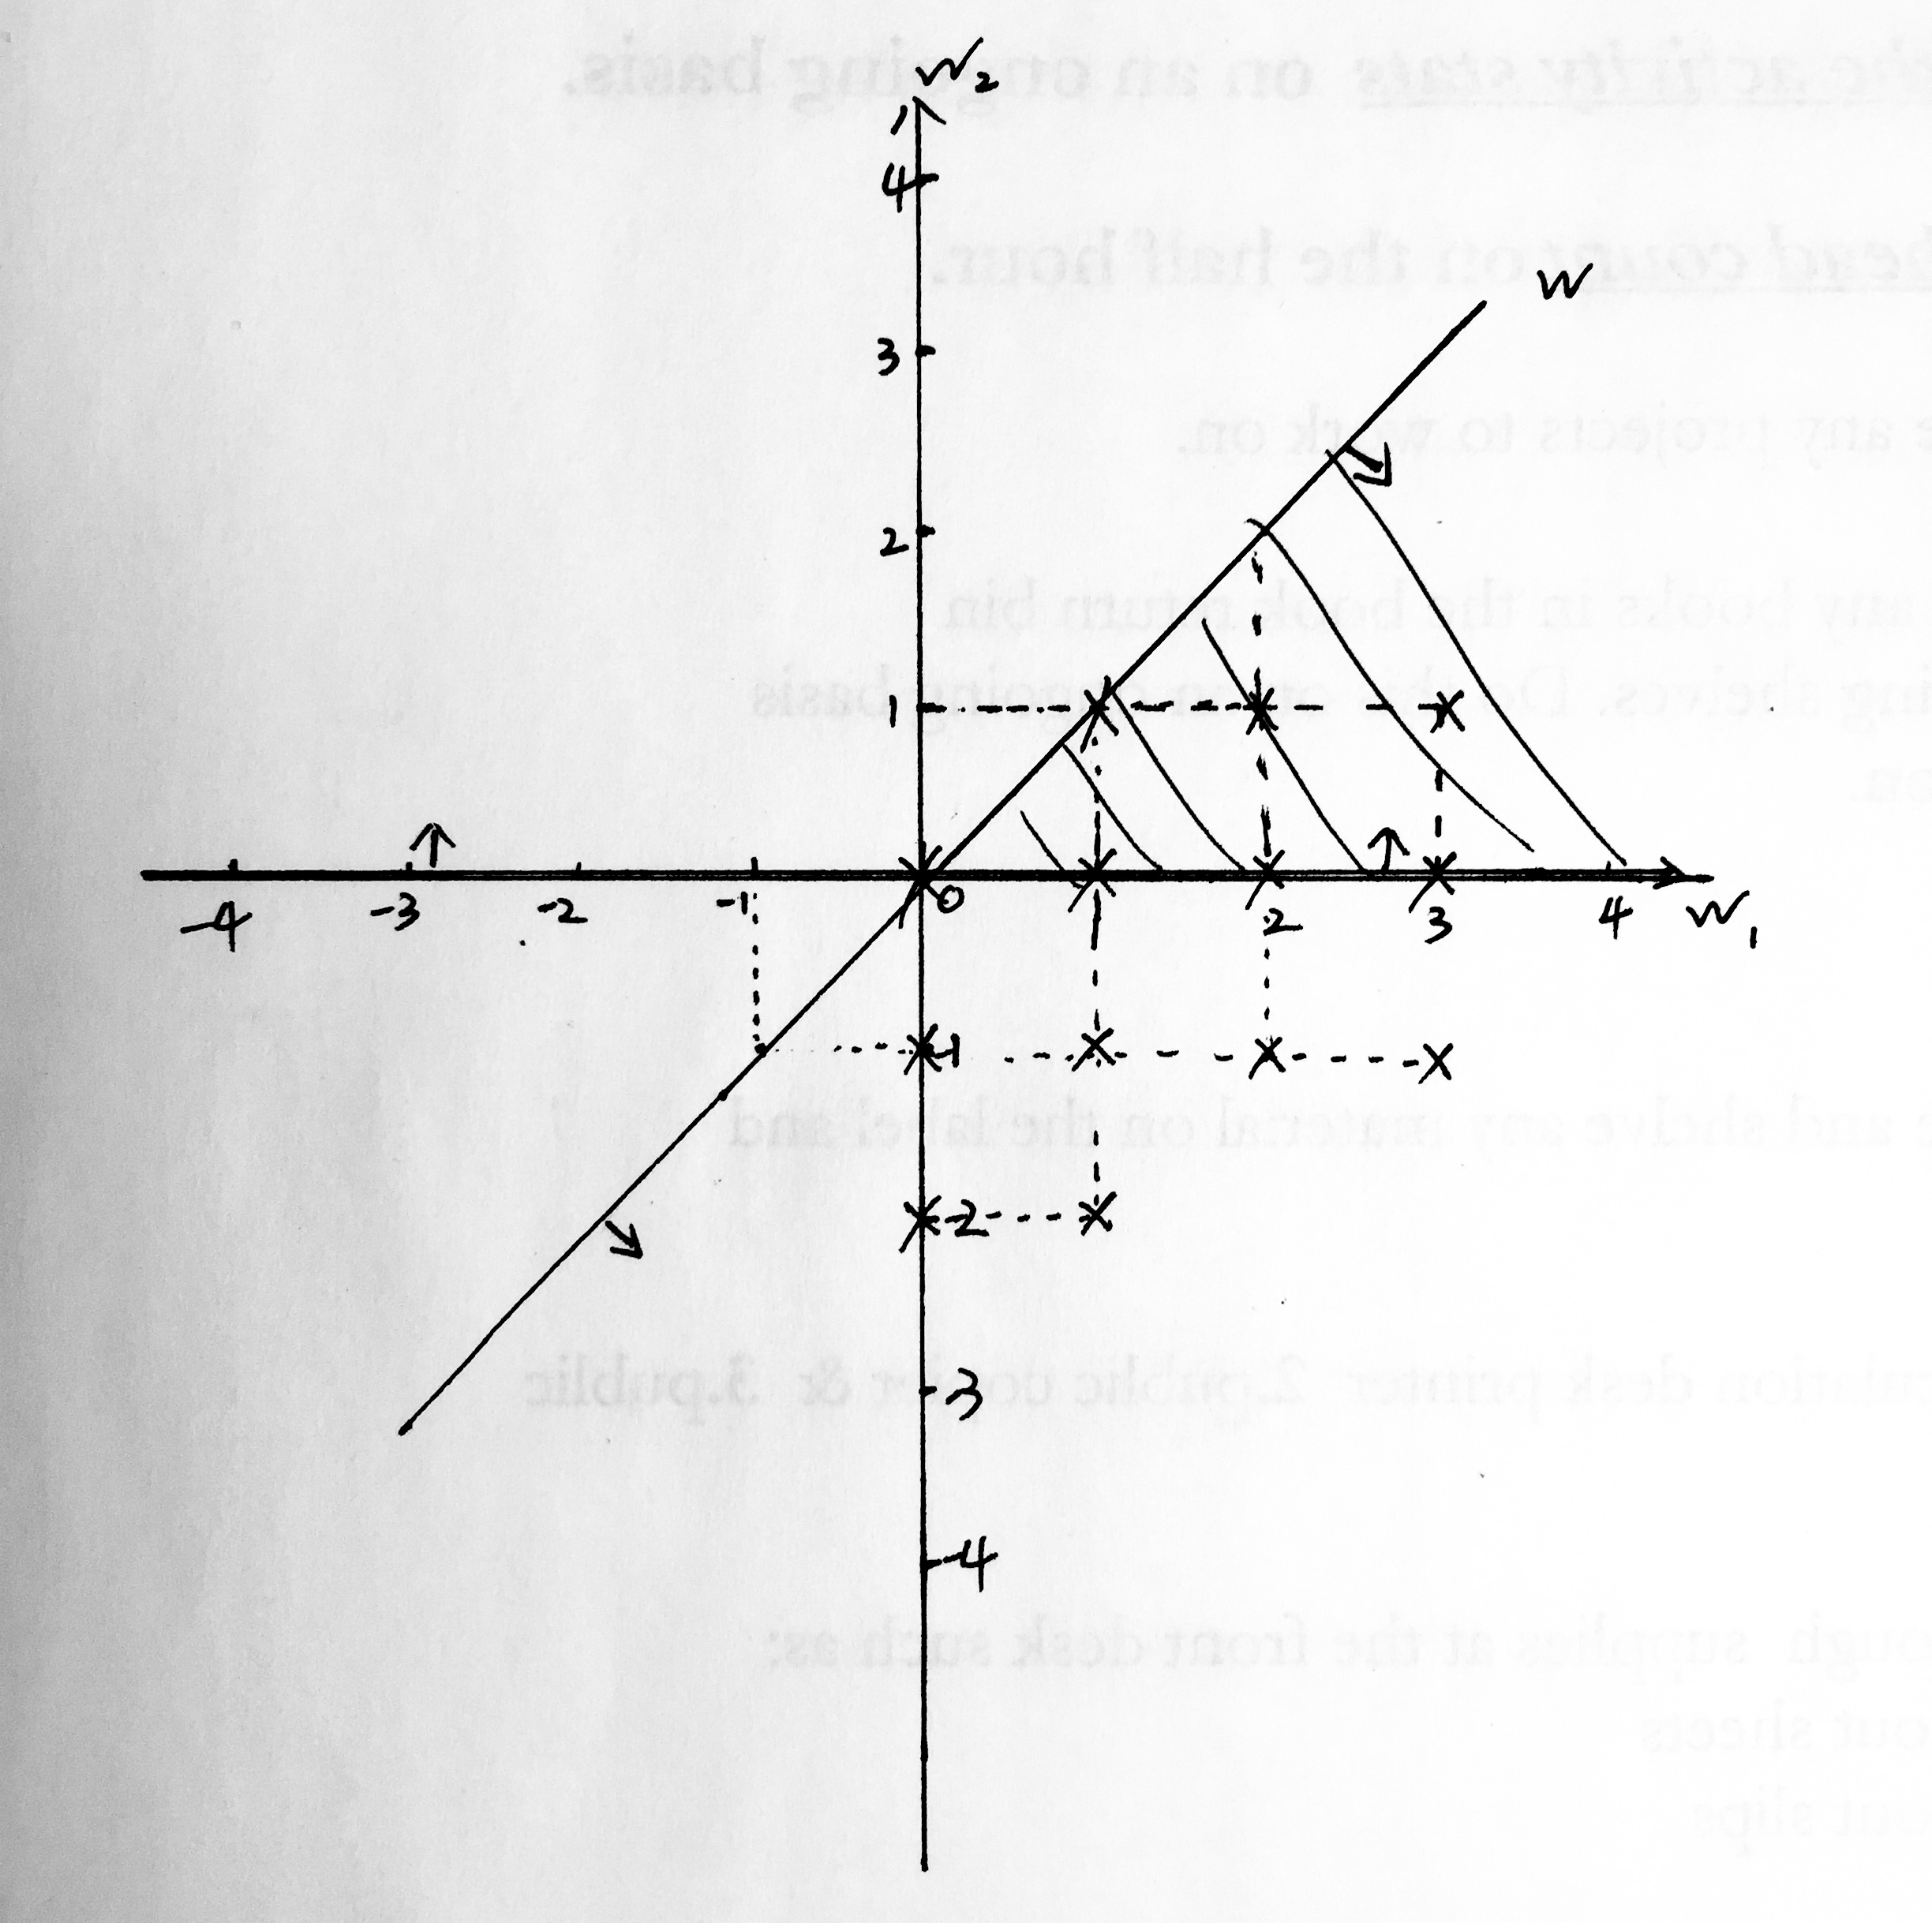
\includegraphics[width=80mm]{1.JPG}
		\caption{1.1 \label{overflow}}
	\end{figure}

%----------------------------------------------------------------------------------------------------------------------
\section*{2}
\begin{enumerate}
	% 2.1
	\item
	$x^{(1)} = -1$ and $t^{(1)} = 1$ implies $w < 0$.\\
	However $x^{(3)} = 3, t^{(3)} = -1$ implies $w > 0$.\\
	Then this dataset is not convex, so it is not linearly separable.
	
	
	%2.2
	\item
	For data $x^{(1)} = -1$, $y^{(1)} = \mathbf{w}^T \boldsymbol{\psi}(x^{(1)}) = -w_1 + w_2 > 0$.\\
	For data $x^{(2)} = 1$, $y^{(2)} = \mathbf{w}^T \boldsymbol{\psi}(x^{(2)}) = w_1 + w_2 < 0$.\\
	For data $x^{(3)} = 3$, $y^{(3)} = \mathbf{w}^T \boldsymbol{\psi}(x^{(3)}) = 3w_1 + 9w_2 > 0$\\
	A pair of values could be $w_1 = -2$ and $w_2 = 1$
\end{enumerate}

%----------------------------------------------------------------------------------------------------------------------
\newpage
\section*{3}

\begin{align*}
\textbf{y} &= \mathbf{Xw} + b\mathbf{1} \\
\dfrac{\partial \mathbf{\mathcal{E}}}{\partial \textbf{y}} &= \dfrac{1}{N} (sin(\mathbf{y} - \mathbf{t})) \\
\dfrac{\partial \mathbf{\mathcal{E}}}{\partial \textbf{w}} &= \dfrac{1}{N} \mathbf{X}^\top sin(\mathbf{y} - \mathbf{t}) \\
\dfrac{\partial \mathbf{\mathcal{E}}}{\partial b} &= \dfrac{1}{N} (sin(\mathbf{y} - \mathbf{t})) \\
\end{align*}

\end{document}
